%% LaTeX2e class for student theses
%% sections/conclusion.tex
%% 
%% Karlsruhe Institute of Technology
%% Institute for Program Structures and Data Organization
%% Chair for Software Design and Quality (SDQ)
%%
%% Dr.-Ing. Erik Burger
%% burger@kit.edu
%%
%% Version 1.1, 2014-11-21

\chapter{Zeitplan und Risikomanagement}
\label{ch:Zeitplan}
In diesem Abschnitt werden das Risikomanagement und der Zeitplan der Bachelorarbeit betrachtet.
\section{Risikomanagement}
Während der Bachelorarbeit müssen mehrere Risiken beachtet werden. \\

Es könnte passieren, dass in der Literatur keine Spezifizierung von Vertraulichkeit sowie deren Anforderung gefunden werden kann. Die Voruntersuchung hat jedoch gezeigt, dass dies unwahrscheinlich ist (vgl. Kapitel \ref{ch:VerwandteArbeiten}). \\

Wahrscheinlicher ist, dass die Modellierung, Implementierung, Validierung sowie das Schreiben der Bachelorarbeit,  mehr Zeit in Anspruch nehmen als geplant. Um dem entgegen zu wirken sollten bei den regelmäßigen Treffen mit den Betreuern die Einhaltung des Zeitplans kontrolliert werden. Dadurch lassen sich Probleme frühzeitig erkennen, Iterationen weglassen und ggf. der Fokus neu setzen lassen. \\

Schließlich könnte der Fall auftreten, dass die geplante Validierung mit Hilfe der Vertraulichkeitsanalyse aus der Arbeit \textbf{Model-Driven Specification and Analysis of Confidentiality in Component-Based Systems} \cite{Kramera} zu aufwendig sein wird, da die Anpassung an die Datenflussmodellierung aus dieser Bachelorarbeit ggf. zu zeitaufwendig ist. Sollte dies der Fall sein, wird mit den Betreuern Rücksprache gehalten und auf die zweite Validierungsmethode zurückgegriffen, die einen geringeren Zeitumfang benötigen wird. 

\section{Zeitplan}
Die Abbildung \ref{abb:zeitplan} zeigt den geplanten Ablauf der Bachelorarbeit. Damit der kontinuierliche Fortschritt der Bachelorarbeit gesichert ist, finden wöchentliche Treffen mit den Betreuern statt.
\newpage
\begin{figure}
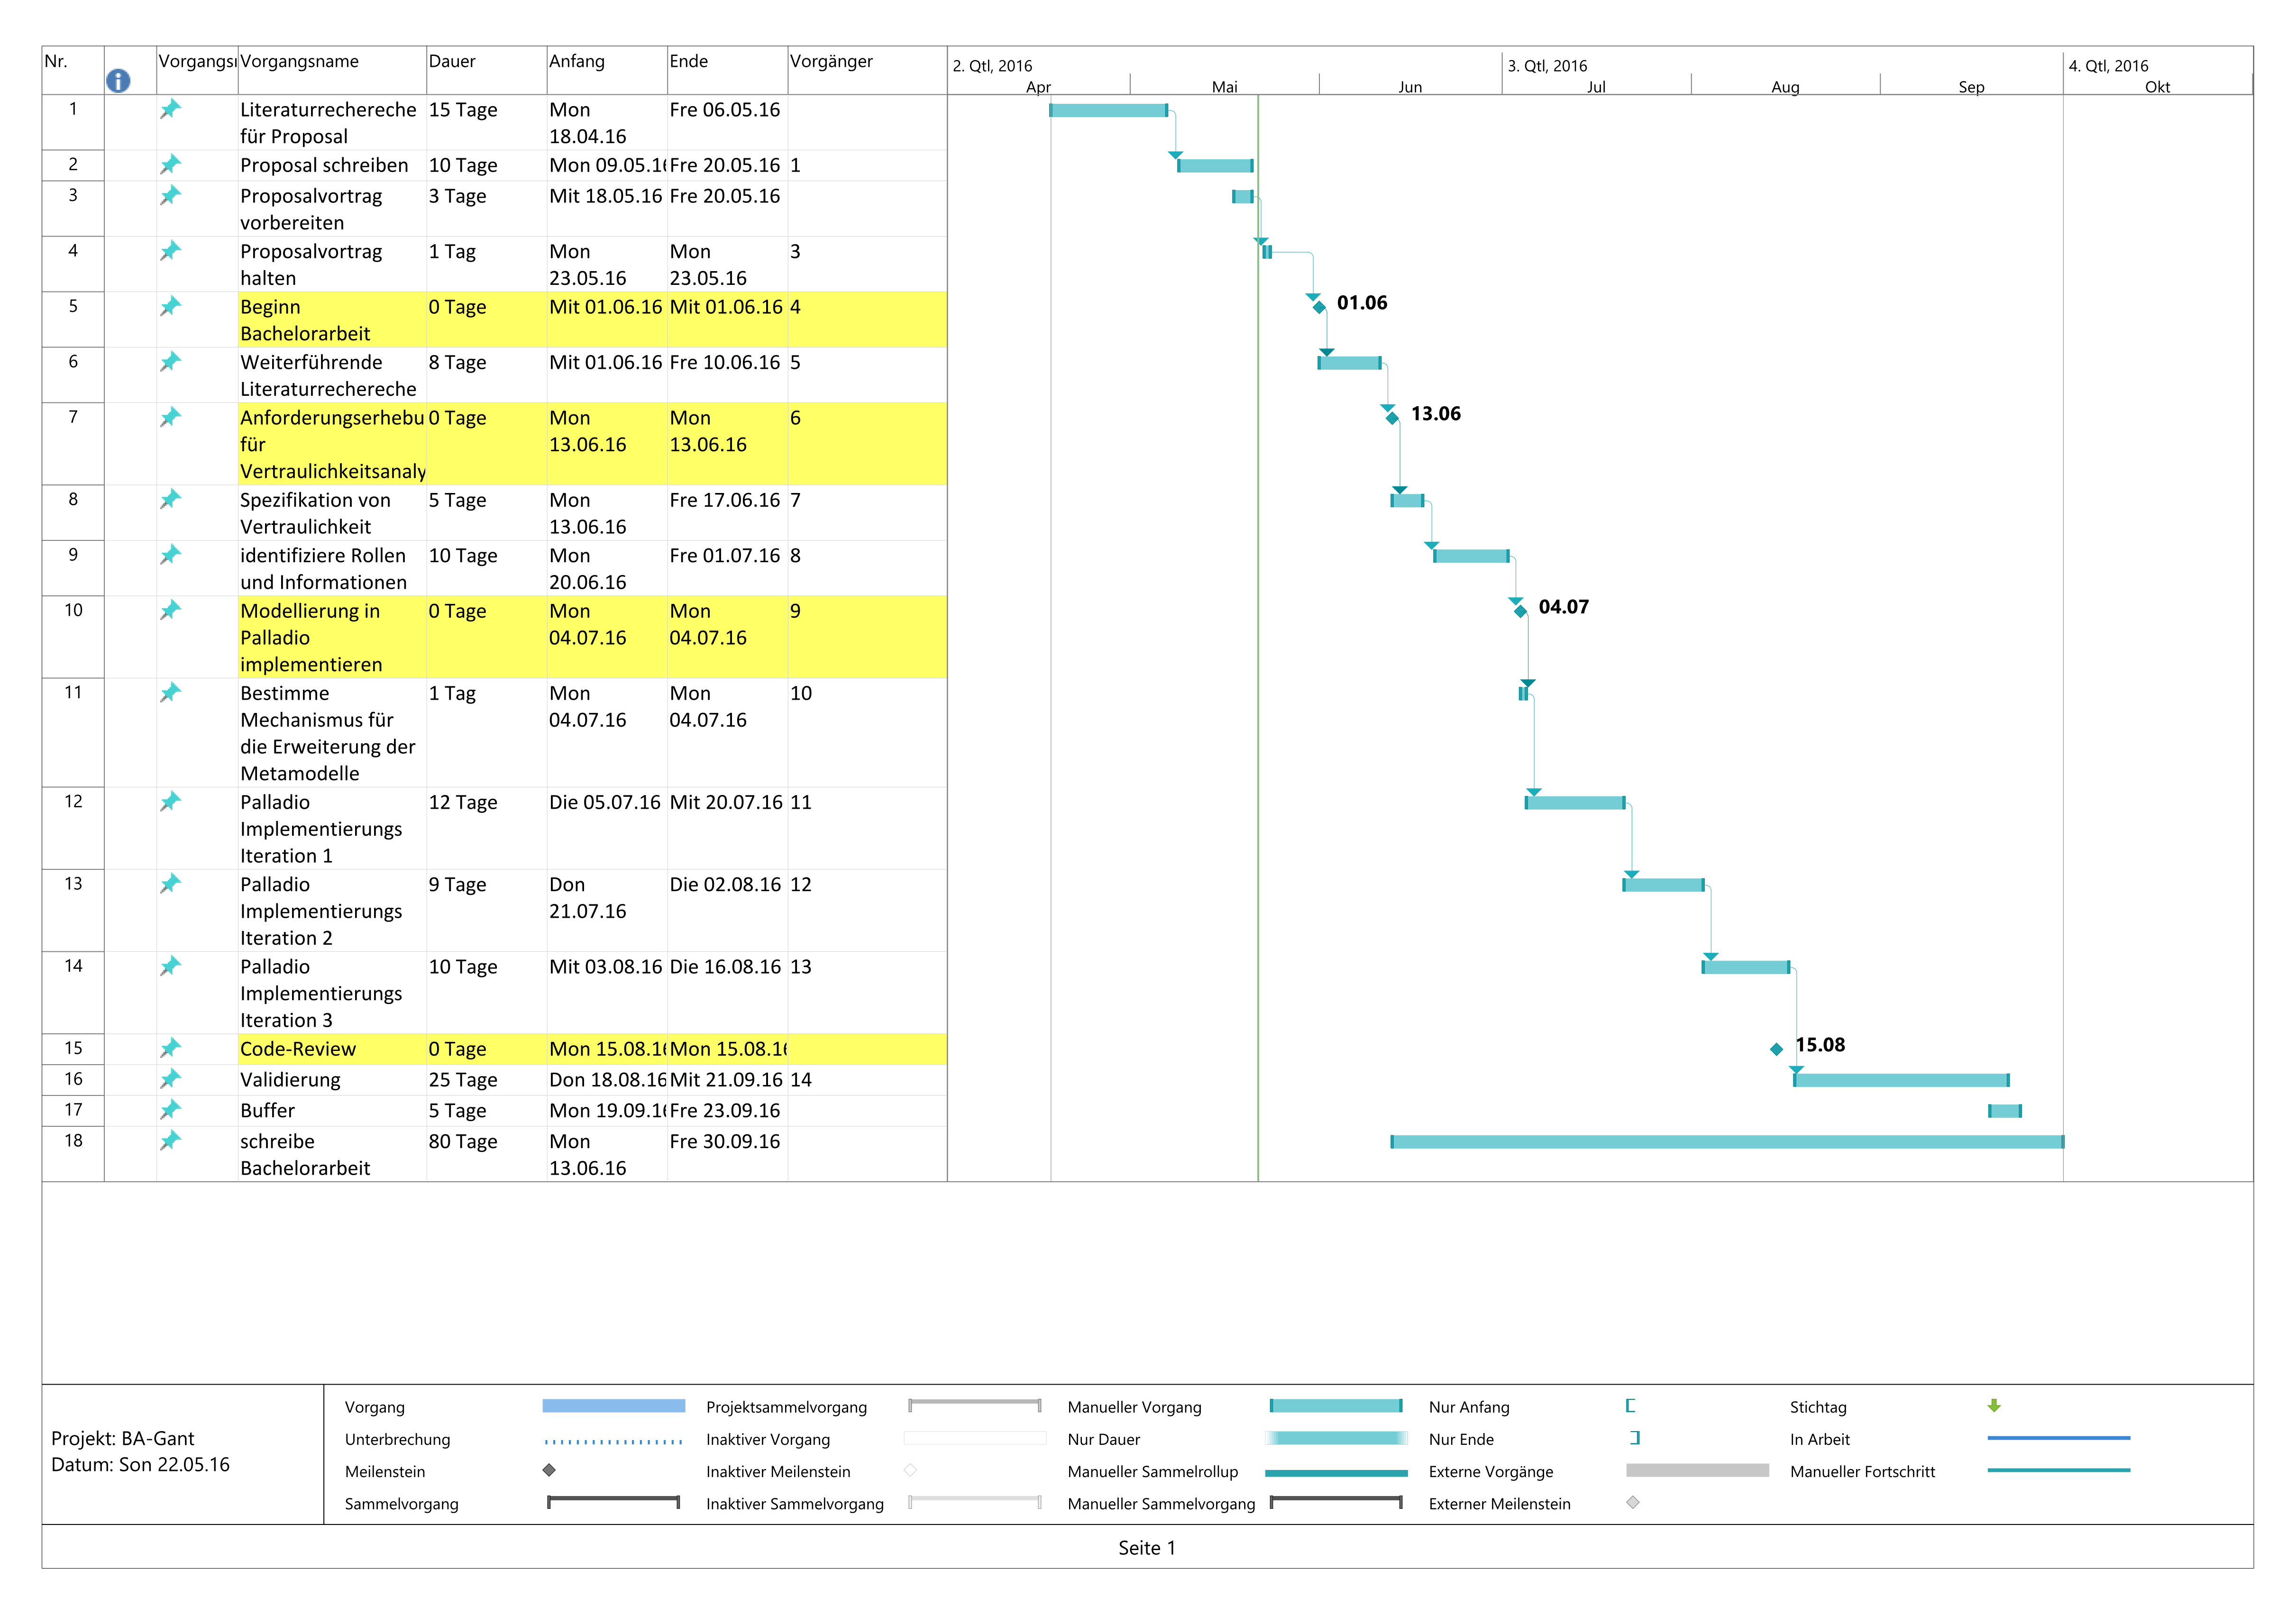
\includegraphics[scale=0.55, angle=90]{images/zeitplan.png}
\label{abb:zeitplan}
\caption{Zeitplan der Bachelorarbeit}
\end{figure}